\section{議論}
近年,学会などでタイムライン表示のテキストチャットが
利用される機会が増えている\cite{wiss_challenge}が、
WISS2009の実証実験\cite{nishida2011}によれば,
全参加者の半分弱しかログインして1回以上発言していなかった.
またWISS2015では,252アカウントが1回以上発言し総発言数は2,948回であったが,
図\ref{powerlaw}のようにアカウントと発言数は冪分布になっており,
発言数上位20\%の50アカウントによる発言が総発言数の78.1\%にあたる2,305回を占めていて,
特定の人ばかりが発言して,発言しない人は全く発言しない傾向が顕著に現れた.

\begin{figure}[h]
\centering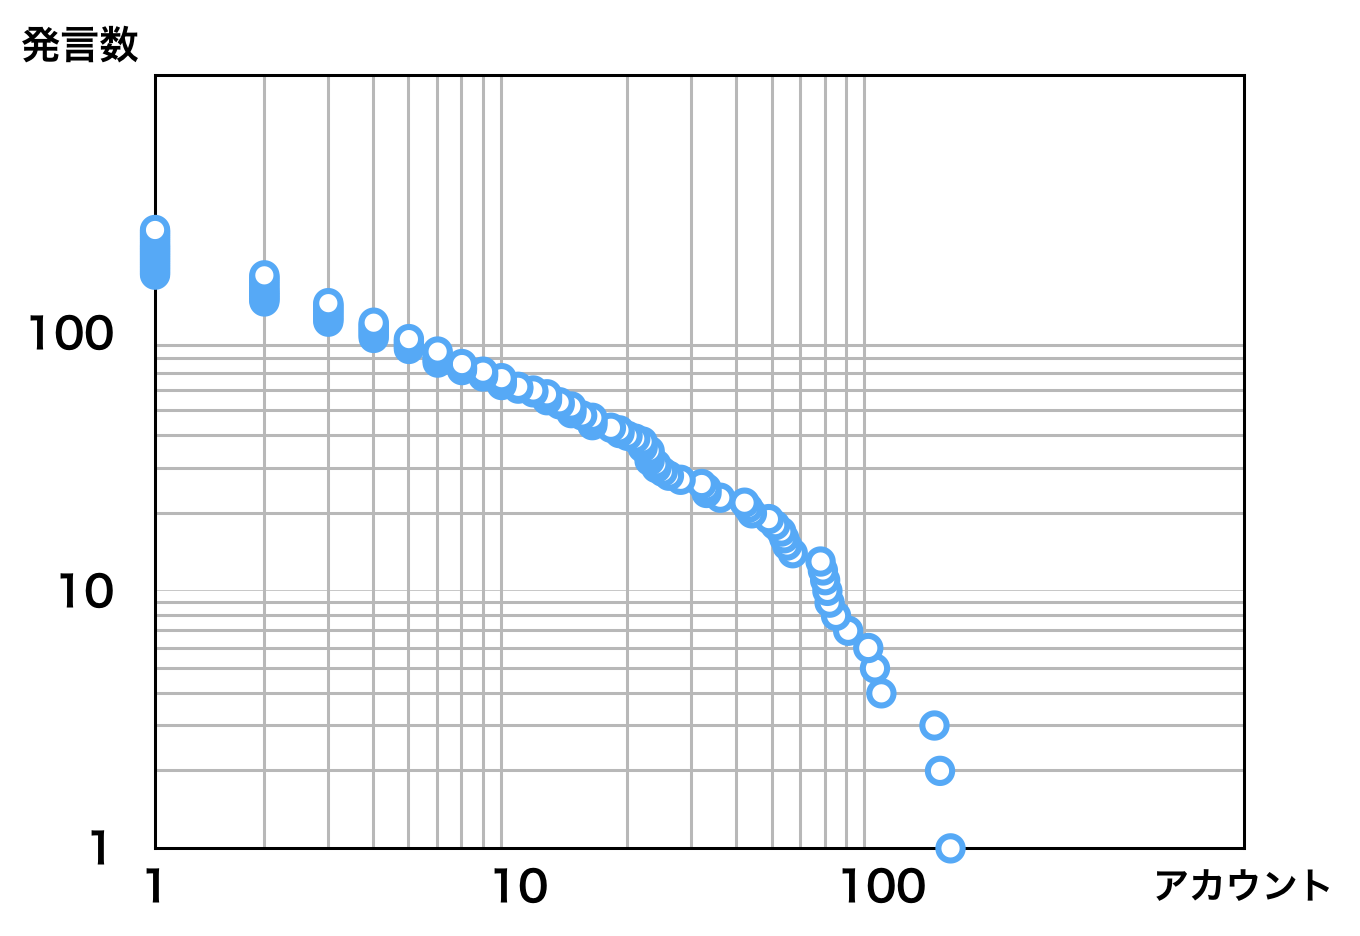
\includegraphics[width=7cm]{images/powerlaw.png}
\caption{WISS2015のチャットのアカウントと発言数の分布の両対数グラフ}
\label{powerlaw}
\end{figure}

『わかるらんど』は長文の高度な発言は期待しておらず,
「なるほど」「わからん」「笑」などといった相槌のようなものを
視覚化してひと目で把握できるようになることを期待している.
本当は議論に参加したいけど声が出ない/手を上げる勇気がない人でも
「なるほど」「わかる」などを『わかるらんど』に投稿することで「参加」することができる.